\documentclass{article}
\usepackage[utf8]{inputenc}
\usepackage[T1]{fontenc}
\usepackage[italian]{babel}
\usepackage{geometry}
\usepackage{graphicx}
\usepackage{amsmath}
\geometry{a4paper, margin=1in}

\title{Capitolo 6 - Controllo degli Accessi}
\author{}
\date{}

\begin{document}

\maketitle

\section*{Fondamenti e Paradigma del Controllo Accessi}

Il controllo degli accessi (AC) riguarda la limitazione di chi può accedere a cosa e in quali modalità. Secondo il paradigma di S. Graham e P. Denning (1972), un soggetto è autorizzato ad accedere a un oggetto esclusivamente in una particolare modalità (access mode), e solo tali accessi autorizzati sono permessi.

\begin{itemize}
    \item \textbf{Soggetto:} È un'entità capace di accedere agli oggetti. Può trattarsi di utenti umani, ma anche di programmi o processi che agiscono per conto degli utenti. I soggetti sono solitamente classificati in tre classi: Proprietario (Owner), Gruppo (Group) e Mondo/Altri (World/Others).
    \item \textbf{Oggetto:} Rappresenta una risorsa su cui viene esercitato il controllo. È un'entità utilizzata per contenere e/o ricevere informazioni, come file, programmi o processi rappresentanti utenti.
    \item \textbf{Modalità di Accesso (Access Mode):} Descrive il modo specifico in cui un soggetto può accedere a un oggetto. Esempi comuni includono:
    \begin{itemize}
        \item \textbf{lettura (Read):} l'utente può visualizzare le informazioni relative a una risorsa di sistema (ad esempio un file). L'accesso in lettura implica la possibilità di copiare o stampare.
        \item \textbf{scrittura (Write):} l'utente può aggiungere, modificare o cancellare dati nelle risorse del sistema (ad esempio, file, record, programmi). L'accesso in scrittura include l'accesso in lettura.
        \item \textbf{esecuzione (Execute):} l'utente può eseguire programmi specifici.
        \item \textbf{eliminazione (Delete):} l'utente può eliminare determinate risorse di sistema, come file o record.
        \item \textbf{creazione (Create):} l'utente può creare file o record.
        \item \textbf{ricerca (Search):} l'utente può visualizzare i file contenuti in una directory o cercare all'interno della directory.
    \end{itemize}
\end{itemize}

\vspace{0.8cm}

\section*{Politiche di Accesso (Access Policies - AP)}

Le politiche di accesso guidano l'implementazione dei meccanismi tecnici. Mentre il \textbf{meccanismo} è facilmente implementabile tramite tabelle e processi informatici (il soggetto può o non può accedere), la \textbf{politica} rappresenta la decisione complessa e sfumata su quali accessi debbano essere consentiti e in quali circostanze.

\subsection*{Obiettivi di Protezione e Monitoraggio}

Le politiche mirano a raggiungere obiettivi di sicurezza fondamentali attraverso il tracciamento e la revisione periodica:

\begin{itemize}
    \item \textbf{Principio del Minimo Privilegio (Least Privilege):} Un soggetto dovrebbe avere accesso solo al numero minimo di oggetti necessari per eseguire un compito specifico. Limitare l'accesso agli oggetti non necessari protegge il sistema da debolezze di sicurezza nel caso in cui una parte del meccanismo di protezione dovesse fallire.
    \item \textbf{Revoca dei Privilegi:} È necessario controllare periodicamente i diritti di accesso per revocare privilegi non più necessari e assicurarsi che tale revoca sia applicata immediatamente.
    \item \textbf{Granularità:} Indica la precisione o specificità del controllo accessi. Una granularità più fine (es. singoli byte in un documento o celle in un foglio di calcolo) comporta un maggior numero di decisioni di controllo e una penalità prestazionale. Tipicamente, l'unità minima di controllo è il file, il programma o uno spazio dati.
    \item \textbf{Audit Log (Registri di Accesso):} I sistemi registrano gli accessi permessi per analisi future. I motivi includono: pianificazione delle risorse, identificazione delle cause di fallimento del sistema, monitoraggio dell'uso improprio da parte degli utenti e analisi delle compromissioni esterne per capire quali dati sono stati rivelati.
    \item \textbf{Privilegio Limitato:} È il concetto gestionale di limitare utenti e processi affinché eventuali danni non siano catastrofici. Si cerca un equilibrio tra la protezione (riservatezza/integrità) e l'utilità/disponibilità del sistema.
\end{itemize}

\vspace{0.8cm}

\section*{Implementazione e il Reference Monitor}

\subsection*{Chi esegue AC}

Il controllo accessi è spesso eseguito dal \textbf{sistema operativo (OS)}, poiché solo esso può accedere a oggetti primitivi come i file e gestire i programmi degli utenti. Tuttavia, l'OS presenta dei limiti: non vede i dati interni alle applicazioni (es. tabelle database), non discrimina facilmente il traffico di rete e l'hardware non sempre supporta controlli a grana fine. Di conseguenza, l'AC è spesso delegato ad applicazioni o apparati di rete.

\subsection*{Reference Monitor}

È un concetto (non uno strumento plug-and-play), su cui dipende l'AC, basato su una combinazione di hardware e software che deve possedere tre proprietà:

\begin{enumerate}
    \item \textbf{Sempre invocato:} Deve validare ogni singolo tentativo di accesso.
    \item \textbf{Immune alla manomissione:} Non deve essere alterabile.
    \item \textbf{Certamente corretto:} Deve esserci la garanzia del suo corretto funzionamento.
\end{enumerate}

\vspace{0.8cm}

\section*{Politiche di controllo degli accessi}

\begin{quote}
    Una politica di controllo degli accessi, che può essere integrata in un database di autorizzazioni, definisce quali tipi di accesso sono consentiti, in quali condizioni e da chi. Le politiche di controllo degli accessi sono generalmente suddivise nelle seguenti categorie:
\end{quote}

\subsection*{1. Controllo degli accessi discrezionale (Discretionary Access Control – DAC)}

\begin{quote}
    è uno schema in cui a un'entità possono essere concessi permessi che le consentono, a suo giudizio, di concedere a un'altra entità permessi di accesso su determinate risorse.
\end{quote}

\subsubsection*{ACM (Access Control Matrix)}

Un approccio generale al DAC, come quello che può essere utilizzato da un sistema operativo o da un sistema per la gestione di basi di dati, consiste in una \textbf{matrice degli accessi}.

La \textbf{Matrice di Controllo Accessi} è un modello astratto che rappresenta i diritti di accesso in una tabella dove le righe corrispondono ai \textbf{soggetti} e le colonne agli \textbf{oggetti}. Ogni cella definisce la modalità di accesso (es. Read, Write, Own) che un determinato soggetto ha su un oggetto specifico.

\vspace{0.5cm}

\noindent \begin{minipage}{0.48\textwidth}
    Poiché l'ACM è solitamente una matrice sparsa (molte celle vuote), può essere rappresentata in modo più efficiente come una \textbf{lista di triple} nella forma \texttt{<soggetto,oggetto,diritti>}. Questa struttura evita di memorizzare celle vuote, ma presenta un problema significativo: la ricerca all'interno di un numero elevato di triple è inefficiente, motivo per cui questa implementazione è raramente utilizzata in pratica.
\end{minipage}
\hfill
\begin{minipage}{0.48\textwidth}
    \centering
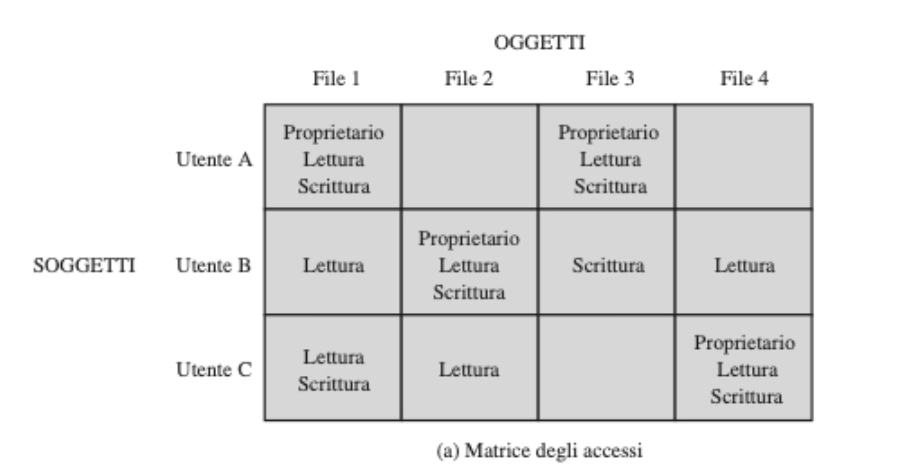
\includegraphics[width=\textwidth]{Screenshot 2026-05-03 alle 17.58.14.png}
\end{minipage}

\vspace{0.8cm}

\subsubsection*{Access Control Directory}

\vspace{0.2cm}
\noindent \begin{minipage}{0.48\textwidth}
Questo approccio consiste nel prendere le righe della matrice ACM e distribuirle tra gli utenti. Viene assunto che ogni file abbia un proprietario unico. Questo proprietario possiede diritti specifici: il diritto di dichiarare chi può accedere al file (e in quale modalità) e il diritto di revocare l'accesso a qualsiasi persona in qualunque momento. In questo modello, esiste una directory specifica per ogni utente che elenca i suoi diritti sulle risorse. Per garantire la sicurezza, a nessun utente è permesso scrivere direttamente nella propria directory di controllo accessi; se ciò fosse possibile, un utente potrebbe falsificare i propri diritti per ottenere l'accesso non autorizzato a un file.
\end{minipage}
\hfill
\begin{minipage}{0.48\textwidth}
    \centering
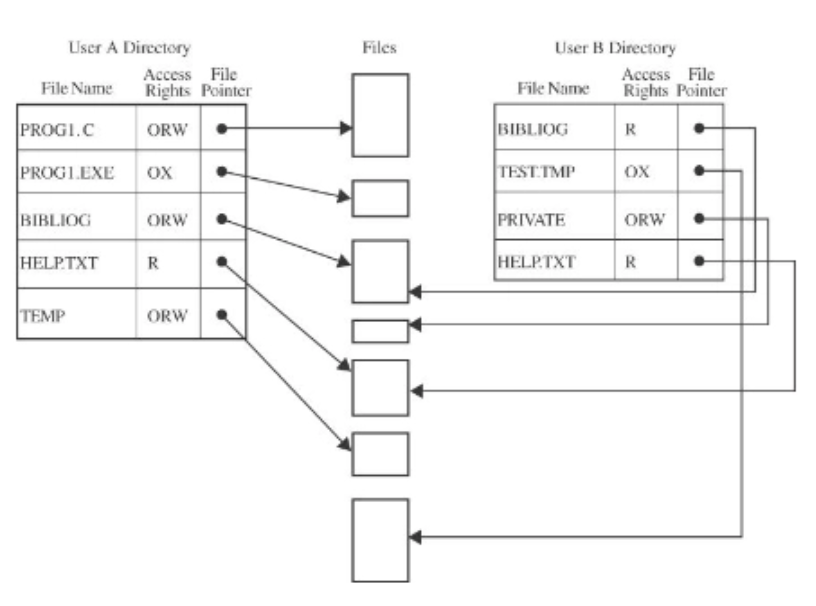
\includegraphics[width=\textwidth]{Screenshot 2026-05-03 alle 17.58.31.png}
\end{minipage}

\vspace{0.5cm}

\begin{itemize}
    \item \textbf{Vantaggi (PRO):} L'implementazione è semplice, poiché consiste in una lista per ogni utente contenente tutti gli oggetti a cui egli può accedere.
    \item \textbf{Svantaggi (CONS):}
    \begin{itemize}
        \item \textbf{Dimensione della lista:} Se ci sono molti oggetti condivisi, la directory può diventare estremamente voluminosa.
        \item \textbf{Revoca dell'accesso:} È un'operazione economica se l'utente A vuole revocare il permesso a B, ma diventa molto costosa se A vuole revocare il permesso a tutti gli utenti contemporaneamente.
        \item \textbf{Propagazione dei diritti:} Se l'utente A concede un permesso a B e B lo trasferisce a C, A potrebbe non esserne a conoscenza (problema della propagazione dei diritti di accesso).
        \item \textbf{Pseudonimi e Rinomina:} Se due utenti diversi chiamano i propri file con lo stesso nome "F", il monitor di riferimento deve gestire l'ambiguità. Inoltre, la rinomina dei file può causare conflitti o permessi inconsistenti.
    \end{itemize}
\end{itemize}

\vspace{0.8cm}

\subsubsection*{Capability}

\vspace{0.2cm}
\noindent \begin{minipage}{0.48\textwidth}
\begin{quote}
    Una \textbf{Capability} è un token non falsificabile che conferisce al possessore determinati diritti su un oggetto. Tecnicamente, è rappresentata come una tripla accessibile solo al sistema, composta da soggetto, oggetto e diritto.
\end{quote}
\end{minipage}
\hfill
\begin{minipage}{0.48\textwidth}
    \centering
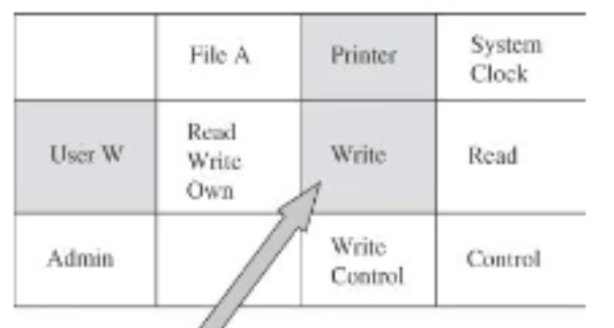
\includegraphics[width=\textwidth]{Screenshot 2026-05-03 alle 17.58.56.png}
\end{minipage}

\vspace{0.5cm}

Esistono due metodi principali per garantire l'integrità delle capability:

\begin{enumerate}
    \item \textbf{Gestione tramite OS:} Il ticket viene consegnato direttamente al sistema operativo (o ai meccanismi di AC) e non all'utente. L'OS mantiene tutti i ticket per conto degli utenti e restituisce all'utente solo un puntatore a una struttura dati interna. Una capability può essere creata solo tramite una richiesta specifica all'OS.
    \item \textbf{Cifratura:} La capability viene cifrata con una chiave disponibile solo all'OS. Se la capability cifrata include l'identità del legittimo proprietario, l'utente A non può copiarla e passarla all'utente B, poiché l'identità non corrisponderebbe.
\end{enumerate}

Con le capability viene introdotto il diritto di \textbf{trasferimento o propagazione}. Un soggetto con questo diritto può passare copie delle proprie capability ad altri soggetti. È possibile limitare la diffusione: ad esempio, il processo A passa una copia a B, ma B può omettere il diritto di trasferimento quando passa la capability a C, impedendo a C di propagarla ulteriormente. Quando un soggetto revoca una capability, non deve essere più permesso alcun accesso tramite essa. Una tabella delle capability può contenere puntatori a tutte le capability "figlie" generate, permettendo all'OS di rintracciarle ed eliminarle.

Le capability sono un modo efficiente per tracciare i diritti durante l'esecuzione. Vengono create a runtime: ogni volta che un processo tenta di usare un nuovo oggetto, l'OS esamina la lista master (ACL o ACM) e, se l'accesso è permesso, genera la capability corrispondente. Devono essere conservate in memoria inaccessibile agli utenti normali:

\begin{itemize}
    \item In segmenti di memoria non puntati dalla tabella dei segmenti dell'utente.
    \item In memoria protetta tramite registri \textit{base/bounds}.
    \item Utilizzando architetture \textit{tagged} che identificano esplicitamente le capability come strutture protette. Durante l'esecuzione, vengono mantenute prontamente disponibili solo le capability degli oggetti effettivamente acceduti dal processo corrente.
\end{itemize}

\vspace{0.8cm}

\subsubsection*{Domini}

\begin{quote}
    Un \textbf{Dominio} è la collezione di oggetti a cui un processo ha accesso in un determinato momento; questa collezione è definita dall'insieme delle capability possedute dal processo. Un esempio pratico è il \textit{namespace} di un processo in Linux.
\end{quote}

Il dominio di una sottoprocedura (SUB) non è necessariamente identico a quello della procedura chiamante (MAIN):

\begin{itemize}
    \item Il chiamante può passare solo alcuni dei suoi oggetti o solo una parte dei suoi diritti di accesso alla sottoprocedura.
    \item La sottoprocedura potrebbe avere accesso a oggetti propri, non accessibili alla procedura chiamante.
\end{itemize}

\vspace{0.8cm}

\subsection*{2. Controllo degli accessi basato sui ruoli (Role-Based Access Control – RBAC):}

\vspace{0.2cm}
\noindent \begin{minipage}{0.48\textwidth}
\begin{quote}
    Il \textbf{Role-Based Access Control (RBAC)} è un modello di controllo degli accessi basato sui \textbf{ruoli} che gli utenti assumono all'interno di un sistema, piuttosto che sulla loro identità individuale. In questo paradigma, un ruolo viene definito come una specifica \textbf{funzione lavorativa} (job function) all'interno di un'organizzazione. A differenza dei modelli tradizionali, i sistemi RBAC assegnano i diritti di accesso direttamente ai ruoli e non ai singoli utenti. Gli utenti vengono poi assegnati a diversi ruoli, in modo statico o dinamico, a seconda delle loro responsabilità operative.
\end{quote}
\end{minipage}
\hfill
\begin{minipage}{0.48\textwidth}
    \centering
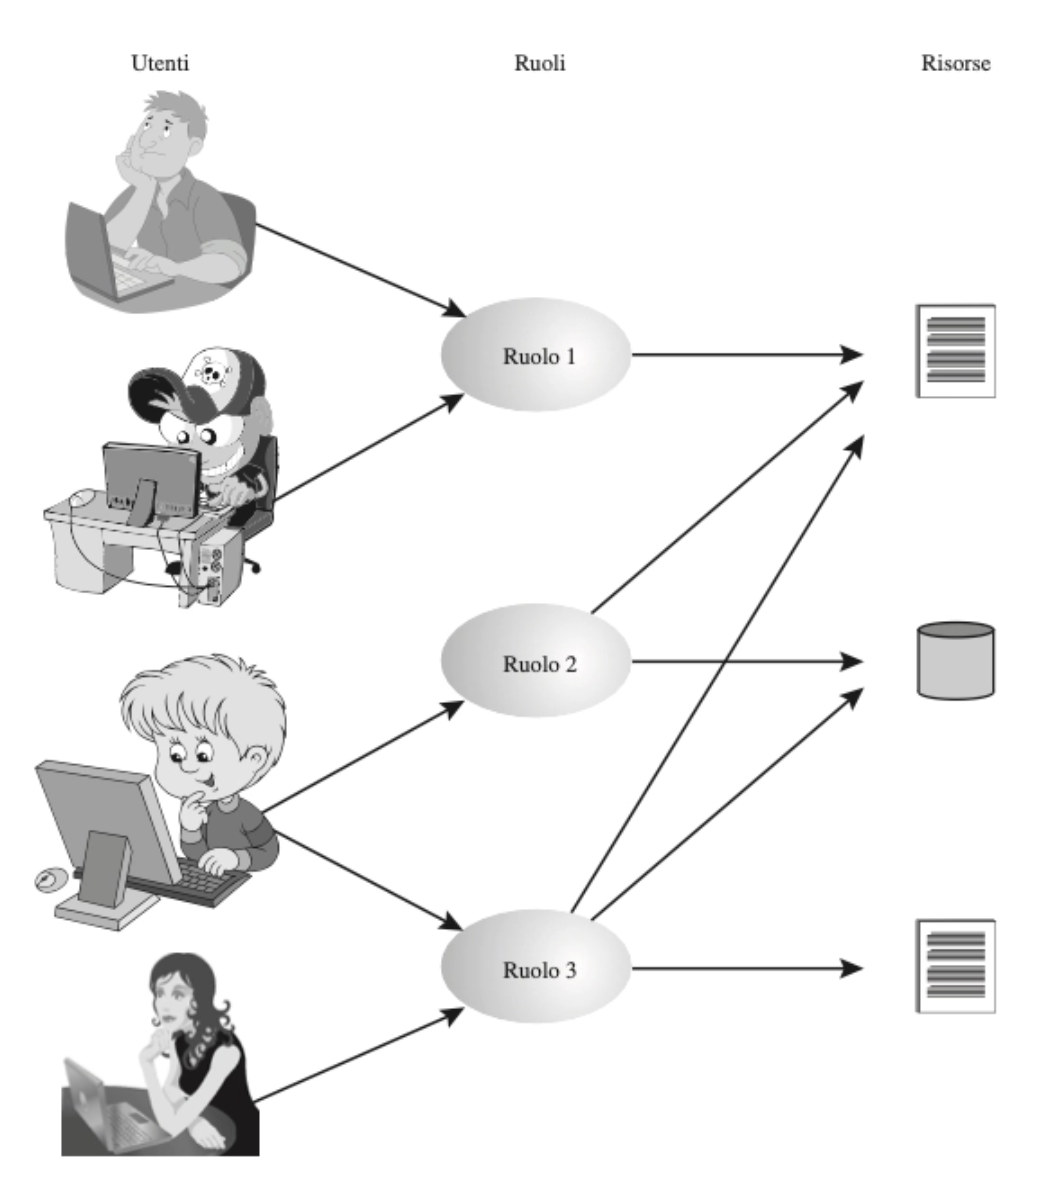
\includegraphics[width=\textwidth]{Screenshot 2026-05-03 alle 17.59.08.png}
\end{minipage}

\vspace{0.5cm}

Il sistema RBAC si adatta a un'efficace implementazione del principio del minimo privilegio. A ogni ruolo dovrebbe essere assegnato l'insieme minimo di privilegi necessari per quel ruolo. Un utente viene assegnato a un ruolo che gli permette di eseguire soltanto ciò che è richiesto per quel ruolo. Gli utenti assegnati allo stesso ruolo godono dello stesso insieme minimo di privilegi.

\vspace{0.5cm}

\subsubsection*{Modelli di riferimento}

Un vincolo è una relazione definita tra i ruoli o una condizione relativa ai ruoli. Si elencano i seguenti tipi di vincoli:

\begin{itemize}
    \item \textbf{Ruoli mutuamente esclusivi:} sono ruoli tali per cui, un utente, può essere assegnato soltanto a un ruolo nell'insieme.
    \item \textbf{Cardinalità:} consiste nell'impostare un numero massimo rispetto ai ruoli. Uno di questi vincoli consiste nel definire il numero massimo di utenti che possono essere assegnati a un determinato ruolo.
    \item \textbf{ruolo prerequisito:} si impone che un utente può essere assegnato a un determinato ruolo solo se è già stato assegnato a un altro determinato ruolo.
\end{itemize}

\begin{itemize}
    \item $RBAC_0$: Rappresenta il modello fondamentale che include utenti, ruoli, permessi e sessioni.
    \item $RBAC_1$: Introduce le gerarchie tra i ruoli, permettendo a un ruolo di ereditare i permessi da un altro.
\end{itemize}

Tipicamente, le funzioni lavorative con maggiore responsabilità possiedono maggiore autorità per accedere alle risorse. Una funzione lavorativa inferiore può, invece, possedere un sottoinsieme dei permessi di accesso della funzione lavorativa superiore. Le gerarchie dei ruoli sfruttano il concetto di ereditarietà, permettendo a un ruolo di includere implicitamente i permessi di accesso associati a un ruolo subordinato.

\begin{itemize}
    \item $RBAC_2$: Introduce dei vincoli che limitano i modi in cui i componenti del sistema RBAC possono essere configurati.
    \item $RBAC_3$: Un modello completo che consolida le caratteristiche delle gerarchie e dei vincoli delle scorse due versioni.
\end{itemize}

\vspace{0.8cm}

\subsection*{3. Controllo degli accessi basato sugli attributi (Attributes-Based-Access-Control – ABAC):}

Il modello \textbf{ABAC} rappresenta l'evoluzione più flessibile e potente dei sistemi di controllo degli accessi. A differenza dei modelli tradizionali, l'ABAC non si limita a verificare chi è l'utente o quale sia il suo ruolo, ma definisce le autorizzazioni attraverso \textbf{espressioni logiche e condizioni} basate sulle proprietà (attributi) sia del soggetto che della risorsa.

Questa metodologia permette di creare regole estremamente granulari. Il suo principale punto di forza è proprio il \textbf{potere espressivo}, che consente di adattare l'accesso a contesti molto specifici. Tuttavia, tale complessità porta con sé una sfida tecnologica: l'impatto sulle prestazioni può essere significativo, poiché il sistema deve valutare predicati complessi su entrambi gli attori (soggetto e oggetto) per ogni singolo tentativo di accesso. Nonostante ciò, l'ABAC ha trovato terreno fertile nei \textbf{servizi Web}, grazie allo standard \textbf{XACML} (eXtensible Access Control Markup Language), e suscita oggi un enorme interesse per la gestione della sicurezza nei \textbf{servizi Cloud}.

\subsubsection*{I Tre Pilastri del Modello: Gli Attributi}

Il cuore del funzionamento dell'ABAC risiede nella capacità di combinare un numero potenzialmente illimitato di attributi per soddisfare qualsiasi regola di sicurezza. Questi attributi si dividono in tre categorie fondamentali:

\vspace{0.3cm}
\noindent \textbf{1. Attributi del Soggetto (Subject Attributes)}

Il soggetto è l'entità attiva che causa il flusso di informazioni o cambia lo stato del sistema. I suoi attributi ne definiscono l'identità e le caratteristiche specifiche. Esempi tipici sono:

\begin{itemize}
    \item \textbf{Ruolo e Titolo lavorativo:} es. "Ingegnere", "Responsabile Vendite".
    \item \textbf{Dipartimento:} es. "Risorse Umane", "Finanza".
    \item \textbf{Livello di autorizzazione (Clearance Level):} fondamentale in contesti militari o governativi per definire il grado di fiducia dell'utente.
\end{itemize}

\vspace{0.3cm}
\noindent \textbf{2. Attributi dell'Oggetto (Object Attributes)}

L'oggetto (o risorsa) è l'entità passiva che contiene o riceve informazioni. Gli attributi dell'oggetto vengono sfruttati dal sistema per prendere decisioni di accesso mirate. Esempi comuni includono:

\begin{itemize}
    \item \textbf{Tipo di file e Sensibilità dei dati:} es. "Documento riservato", "File di sistema".
    \item \textbf{Proprietario:} l'identità di chi ha creato o gestisce la risorsa.
    \item \textbf{Associazione al progetto:} permette di limitare l'accesso solo ai membri di uno specifico team di lavoro.
\end{itemize}

\vspace{0.3cm}
\noindent \textbf{3. Attributi dell'Ambiente (Environment Attributes)}

Questa categoria descrive il contesto operativo, tecnico o situazionale in cui avviene la richiesta di accesso. È l'elemento che differenzia maggiormente l'ABAC dagli altri modelli, poiché permette di inserire variabili esterne alla relazione diretta utente-risorsa.

\begin{itemize}
    \item \textbf{Parametri temporali:} es. orario della richiesta, giorno della settimana.
    \item \textbf{Sicurezza della rete:} es. livello di protezione della connessione utilizzata.
    \item \textbf{Posizione geografica:} es. accesso consentito solo se l'utente si trova fisicamente in ufficio.
\end{itemize}

\vspace{0.8cm}

\subsubsection*{Architettura e Logica di Valutazione}

Il funzionamento logico dell'ABAC si distingue perché valuta le richieste di accesso non contro una semplice lista di nomi, ma contro un insieme di \textbf{regole di controllo (Access Control Policies)} che definiscono le operazioni permesse per specifiche combinazioni di attributi in un dato ambiente.

Secondo lo scenario standard dell'ABAC, il processo si articola in tre fasi principali:

\begin{enumerate}
    \item \textbf{Richiesta:} Un utente (soggetto) tenta di eseguire un'operazione su una risorsa.
    \item \textbf{Meccanismo di Controllo:} Il sistema recupera le policy di accesso e interroga i database degli attributi per raccogliere i dati relativi al soggetto, all'oggetto e all'ambiente corrente.
    \item \textbf{Decisione:} Attraverso la valutazione logica di questi elementi, il sistema emette un verdetto finale: \textbf{Permit} (Accesso consentito) o \textbf{Deny} (Accesso negato).
\end{enumerate}

\vspace{0.5cm}

\subsubsection*{Scenari ed Esempi Pratici}

L'efficacia dell'ABAC è meglio comprensibile attraverso esempi di applicazione dinamica che i modelli tradizionali (come il RBAC) farebbero fatica a gestire senza un'enorme proliferazione di ruoli:

\begin{itemize}
    \item \textbf{Accesso Temporale:} Un dipendente del settore vendite può modificare i record CRM dei clienti solo se l'orario corrente è compreso tra le 08:00 e le 18:00.
    \item \textbf{Controllo basato sulla Posizione:} Un dipendente può accedere ai "Dati Sensibili" solo se la sua posizione di connessione è identificata come "Rete Aziendale Interna".
    \item \textbf{Approvazione di Transazioni Finanziarie:} Un analista può approvare un trasferimento di denaro solo se il valore della transazione è inferiore al suo limite personale di autorizzazione.
    \item \textbf{Accesso per Consulenti Esterni:} Un consulente può accedere a un documento solo se il suo stato lavorativo è "Contractor" e l'accesso è permesso solo fino alla "Data di Scadenza" del contratto (attributo ambientale).
    \item \textbf{Visibilità dei Dati Regionale:} Un dipendente di una sede regionale può visualizzare le righe di un database solo se il "Tag della Regione" sui dati corrisponde al proprio attributo regionale (es. "EMEA").
\end{itemize}

\end{document}